% !TEX root = ../presentation.tex
% !BIB program = biber
% !TEX program = xelatex

\section{discussion}

% - It could be interesting to discuss the remaining challenges in integrating the thesis’ range of topics into multi-stage systems for medical domains. This reflects a recurring pattern of clear intra-chapter content, and it would be interesting to discuss further the integration across thesis parts.


% Chapter 4:
% - a point for elaboration of this work would for it to be more prescriptive about how to choose the value of k in the ratio statistic, as it seems to be quite a crucial hyperparameter for practical implementation.

% Chapter 6:
% - Schematically, Figures 6.1 and 6.2 seem inconsistent and could support the text more through a consistent use of colours and labels between them.
% - The chapter doesn’t answer the pressing questions from Chapter 10: What about self-supervised methods for downstream tasks, and should one abandon ship and only focus on self-supervised methods? – this would be interesting to discuss.


\begin{frame}
    \frametitle{The broad picture: The field of AI since 2020}
    \begin{itemize}
        \item <1-> [2020] \textbf{Project start}
        \begin{itemize} 
            \item <1-> Out-of-distribution detection with generative models: Mysterious new topic.
            \item <1-> Speech recognition: Inflection point between supervised methods and dawning self-supervised approaches.
            \item <1-> Large language models such as BERT and GPT were becoming popular for fine-tuning on specific tasks.
        \end{itemize}
        \item <2-> [2024] \textbf{Project end}
        \begin{itemize}
            \item <2-> Out-of-distribution detection is a mature field with a wide range of methods.
            \item <2-> Self-supervised learning is the dominant paradigm in speech recognition.
            \item <2-> Large language models are a commodity and the paradigm of fine-tuning for instruction (RLFH/DPO \cite{ouyang_training_2022,rafailov_direct_2024}) has fundamentally changed how they are used.
        \end{itemize}
    \end{itemize}
\end{frame}


\begin{frame}
    \frametitle{The role of uncertainty in an operational decision support system}
    \begin{columns}
        \begin{column}{0.6\textwidth}
            \begin{itemize}
                \item Do we need true uncertainty estimates? Pragmatism versus idealism.
                \item Role of explainability compared to uncertainty estimates. 
                \item European Parliamentary Research Services \cite{europeanparliament_artificial_2022}:
            \end{itemize}
            \vspace{0.5em}
            \begin{center}
                {\itshape "Future AI solutions for healthcare should be implemented by integrating uncertainty estimation, a relatively new field of research that aims to provide clinicians with clinically useful indications on the degree of confidence in AI predictions"}
            \end{center}
        \end{column}
        \begin{column}{0.4\textwidth}
            \vspace{-2em}
            \begin{figure}[t]
                \centering
                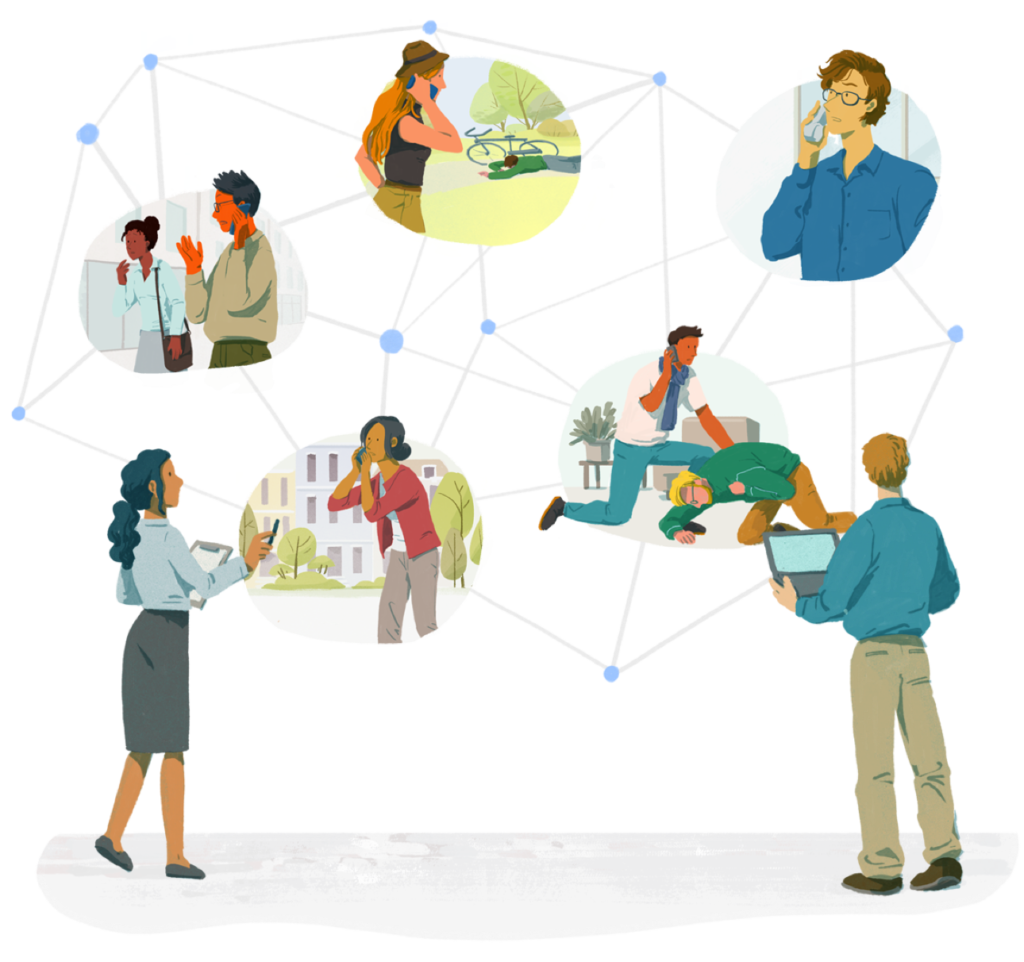
\includegraphics[width=0.9\textwidth]{figures/corti_sketch_conversations.png}
            \end{figure}
        \end{column}
    \end{columns}

\end{frame}


\begin{frame}
    \frametitle{What lies ahead}

    Self-supervised learning in the wild:
    \begin{itemize}
        \item A single emergency service can store hundreds of thousands of calls with rich metadata every year. Does the recent progress on academic datasets translate to this real-world setting?
    \end{itemize}
    % \begin{itemize}
    %     \item <1-> \textbf{Out-of-distribution detection}
    %     \begin{itemize}
            
    %     \end{itemize}

\end{frame}


% \textbf{From global to local} In table 1, we see that work on global representations within self-supervised learning pre- cedes work on local representations. However, we find that the core ideas underlying the recent successes in learning lo- cal representation models have also been used for global rep- resentation learning; masking (Chung et al. 2016), context prediction (Chung and Glass 2018), and contrastive train- ing (Milde and Biemann 2018) have been applied in both settings. Furthermore, where work on global representa- tion learning has taken inspiration from Word2vec (Mikolov et al. 2013), the techniques used for learning local repre- sentations are inspired by contextualized word embeddings (Devlin et al. 2019). Thus, the gap between these two model classes is largely a product of the developments in related fields and the general increase in computational resources.

% \textbf{Representations beyond inference} Predictive tasks are commonly used for self-supervised models, but they are not directly compatible with LVM training. However, an LVM prior with an autoregressive parameterization, p(zt|z1:t−1) or p(zt|x1:t−1), can be seen as predictive in the sense that it tries to match the approximate posterior. Hence, the prior might be considered for feature extraction. Jones and Moore (2020) examine the importance of the prior in the VQ-VAE and show that the ability of this model to estimate den- sities p(x1:T ) lies solely in its prior. Other work has also explored representations beyond the latent variable such as hidden units of the observation model (Khurana et al. 2020; Chorowski et al. 2019b).

% \textbf{Masking and missing data} Masking may also improve representations learned with VAEs. Masking in VAEs has already been explored in the literature in the context of miss- ing data imputation. Here, x is only partially observed, and often represented as a segmentation into observed and miss- ing parts and a mask m indicating where the data is missing. The model is then trained to infer the latent variable from the observed data. Reconstruction also deals only with the ob- served data. Previous work has largely focused on the abil- ity of these models to yield high-quality imputations within the tabular and image data domains, without probing for the effects on the learned latent representation (Mattei and Frellsen 2019; Ipsen, Mattei, and Frellsen 2021). The idea of using VAEs to impute missing data was already examined in the seminal paper by Rezende, Mohamed, and Wierstra (2014). Here the model was trained with fully observed data and used to impute data in an iterative sampling approach post hoc leaving the learned representations unchanged.

% \textbf{Evaluating representations} Although this review has a primarily methodological focus, we should briefly touch upon evaluation procedures. Training metrics for self- supervised tasks and the likelihood of LVMs offer little guid- ance as to the quality of the learned representations (Husza ́r 2017). Thus, a common approach is to evaluate the repre- sentations in terms of their usefulness for downstream tasks. Such tasks may be chosen to target specific attributes of the representation (e.g. semantic or speaker information).

% The SUPERB benchmark (Yang et al. 2021) gathers mul- tiple tasks grouped into categories such as recognition, de- tection, semantics, speaker, paralinguistics and generation. The recently proposed SLUE benchmark focuses on spo- ken language understanding (Shon et al. 2021). The long- standing zero resource speech challenge (ZeroSpeech) offers a new set of tasks for each edition (Versteegh et al. 2015; Dunbar et al. 2017, 2019, 2020, 2021) usually featuring a minimal-pair ABX task (Schatz et al. 2013, 2014).

% Tasks that evaluate representations in terms of speaker- related information include speaker verification (Hsu, Zhang, and Glass 2017b; Khurana et al. 2019; Milde and Biemann 2018), speaker identification (van den Oord, Li, and Vinyals 2018; Jati and Georgiou 2019; Chung et al. 2019; Liu, Chung, and Glass 2021), dialect classification (Khurana et al. 2019), emotion recognition (Pascual et al. 2019; Yang et al. 2021) and gender classification (Lee et al. 2009). The semantic content of representations are evaluated using tasks such as intent classification (Morais et al. 2021; Yang et al. 2021), slot filling (Lai et al. 2021; Yang et al. 2021), sentiment analysis (Liu et al. 2020), question answer- ing (Chung, Zhu, and Zeng 2020), named entity recogni- tion (Shon et al. 2021; Borgholt et al. 2021a; Pasad et al. 2021) and speech translation (Bansal et al. 2017; Chung and Glass 2020a). Cardiac arrest detection for emergency calls has also been used to evaluate speech representations (Borgholt et al. 2021a). For local representations, phoneme classification is very common (Lee et al. 2009; Hsu, Zhang, and Glass 2017a; Chorowski et al. 2019b; Chung et al. 2019; Liu, Li, and Lee 2021). However, automatic speech recogni- tion has become the de facto standard benchmark task (Ling and Liu 2020; Chung and Glass 2020a; Hsu et al. 2021).

% \textbf{Moving forward} Most of the seminal work has focused on improving speech recognition (Schneider et al. 2019; Baevski et al. 2020). This focus has gained traction over the last couple of years, as computational resources have be- come more accessible and end-to-end models (Graves et al. 2006; Chan et al. 2016) have been established as the dom- inant approach to speech recognition (Gulati et al. 2020). It is important to stress that self-supervised models, such as wav2vec 2.0 (Baevski et al. 2020), represent a breakthrough, and recent successful approaches build upon this method. That is, deep self-attention models combined with masking (Hsu et al. 2021; Wang et al. 2021; Chen et al. 2021). This development mirrors years of rapid progress in masked lan- guage modeling within natural language processing (Devlin et al. 2019; Clark et al. 2020) and we expect this to continue for unsupervised neural speech representation learning.
